\vssub
\subsubsection{~三角形非结构网格} \label{sub:num_space_tri}
\conthead{WWM-II}{A. Roland, F. Ardhuin, M. Dutour-Sikiri\'c, A. Abdolali}

\noindent
在 \ws\ 中，可以选择基于三角形的非结构网格，并使用基于轮廓残差分配（CRD）的数值格式 \citep{art:ricchiuto2005} 来离散空间导数。这些格式已在 \citep{rep:Roland2008} 中应用到波作用量平衡方程，并在 Wind Wave Model-II (WWM-II) 和 WW-III 中实现。对于时间积分方法，非结构网格可使用显式和隐式格式。如果选择显式求解器，则使用 WW3 原始分步法，其中地理空间中二维双曲部分的解在非结构网格上用上述方法求解。在这种情况下，谱部分和源项的积分方式与 WW3 结构网格版本类似。时间步长定义也与结构网格部分相同，只是非结构部分的子迭代次数会根据区域内最大 CFL 数自动估计。若选择隐式方法，则根据 \citep{rep:Roland2008}，基于 CRD-N 格式组装线性方程组。谱传播部分用简单的隐式一阶迎风格式求解，源项则以与 WW3 动态格式相同的方式写入矩阵，即在式 3.61 中取 $\epsilon = 1$，并按简单 Patankar 规则组装方程组。新实现的完整说明见 \cite{rolandetal2019t}。可以通过解析推导和数值实验表明，当 CFL \textless 1 时，显式和隐式方法给出相似结果。这也已在实际应用中得到展示，例如 \citep{rep:Abdolalli2018, Smith2018, rep:Abdolalli2019, AbdolaliEtAl2019OM}。不过，当 CFL \textgreater 1 时，由于源项在时间上线性化，隐式格式的瞬态解具有时间步长依赖性。隐式格式中的时间步长等于全局时间步长，谱空间或源项的其他时间步长不起作用。分步法同样由于分裂误差而具有时间步长依赖性，这在浅水中尤为显著 \citep{rep:Roland2008}。对于两类数值方法，除非给定应用的精度水平已经令人满意，否则都需要针对全局时间步长和空间分辨率进行适当的收敛性分析。随后，这些数值实现已在 WWIII 中得到评估 \citep[e.g.][]{art:Aea09,art:babanin2011,art:bertin2014,
art:bertin2015,art:dodet2013,art:ferrarin2008,art:ferrarin2013,art:janekovic2015,art:kerr2013,art:liau2011,art:Mea10,art:perrie2018,
art:perrie2013two,pro:rol2006a,pro:rol2006b,art:rol2009,art:rol2012,art:rol2014,art:sikiric2012,art:sikiric2013,art:sikiric2018,
pro:zanke2006}。


该选项通过在 {\file ww3\_grid.inp} 中把网格字符串设为 `{\code UNST}' 激活。已实现四种格式，具体选择通过 {\code UNST} namelist 完成。它们是 CRD-N 格式（一阶）、CRD-PSI 格式（优于一阶，在三角形结构网格上为二阶）、CRD-FCT 格式（二阶时空格式）和隐式 N 格式。默认格式是效率最高但扩散较强的显式 N 格式。RD 格式的一种隐式变体使用直线法和 N 格式进行空间离散，该方法由 \cite{art:Zij10} 在 SWAN 模式中实现；ECWAM 当前版本采用了类似离散，见 \cite{pro:rol2012}。

在这种方法中，节点处谱的演变（谱也在节点处求值）基于把进入与节点相关的中位对偶单元的通量收敛重新分配到节点上（见图 \ref{fig:triangles}）。对任意谱分量，平流方程式 (\ref{eq:step_xy_prop}) 在中位对偶单元上求解：进入一个单元的通量给出相应节点处波作用量的变化率。已实现的不同格式在估计该通量时采用不同离散。相关格式已在 \citep[见][综述]{rep:Roland2008} 中介绍。

需要注意的是，这些平流格式不包括 garden sprinkler effect (GSE) 修正。按照通常意义上的 GSE 修正，已发现 N 格式具有足够的数值横向扩散，可很好地补偿该效应。然而，CRD-PSI 或 CRD-FCT 等高阶格式可能根据空间分辨率产生显著 GSE 影响。

非结构网格格式的并行化可以采用与结构网格相同的 Card Deck 方法，也可以使用区域分解方法。区域分解方法基于 ParMetis \citep{rep:karypis2011metis}，后者是并行图划分算法的 C 实现。ParMetis 通过 Fortran 中的 PDLIB（Parallel Decomposition Library）接口调用；除连接 ParMetis 外，PDLIB 还按照 Fortran2002 标准提供非结构网格所需的交换例程。交换例程根据 ParMetis 提供的分解，在分解网格的不同线程之间执行所有所需通信。这样，所有区域分解部分只需一行代码即可并入主源码。要在开关文件中编译 PDLIB 选项以激活区域分解并行化，需要安装 ParMetis，并且代码需要使用 MPI 编译。PDLIB 可与所有常见 MPI 实现配合工作，例如 OpenMPI、MPICH2 等。WW3 中已实现并行算法（card deck 和区域分解）的示意图见图 \ref{DDvsCD}。对于实际应用，\cite{AbdolaliEtAl2019OM} 在 2008 年 Hurricane Ike 案例中展示了这两种方法的收敛性。

在实际中，可使用 PolyMesh 软件（由 Aron Roland 开发）由岸线多边形数据库和任意测深点列表轻松生成非结构网格。PolyMesh 连接 Triangle，并采用基于波浪传播特征的先验误差估计，以及基于重心法水深误差的深度误差估计 \citep[e.g.][]{art:WS96}。也可使用 SMS 和 OceanMesh2D 等其他网格生成工具。对三角形形状没有约束。

规则网格显式有限差分格式中 CFL 条件的等价量，是对偶单元面积除以时间步长与进入对偶单元的正波动之和的乘积。由于正通量的谱值在边界上强制给定，边界节点被排除在该 CFL 计算之外，入射能量设为零，而出射能量完全吸收。只有反射部分允许能量从边界进入区域。

岸线处的边界条件取决于波向相对于岸线取向的关系。该特殊处理通过 `{\code IOBPD}' 数组强制执行；每当网格点状态图 `{\code MAPSTA}' 改变时，该数组会更新。网格几何还用于定义局地水深和流的梯度。所有其他操作，例如把强迫插值到网格上，以及从网格插值到输出位置，均使用三角形内线性插值完成。

所有三角形几何操作都假定局地地球为平面。网格上的水深和流梯度在节点处估计，方法是在一个三角形内用线性形函数插值。

\begin{figure} \begin{center}
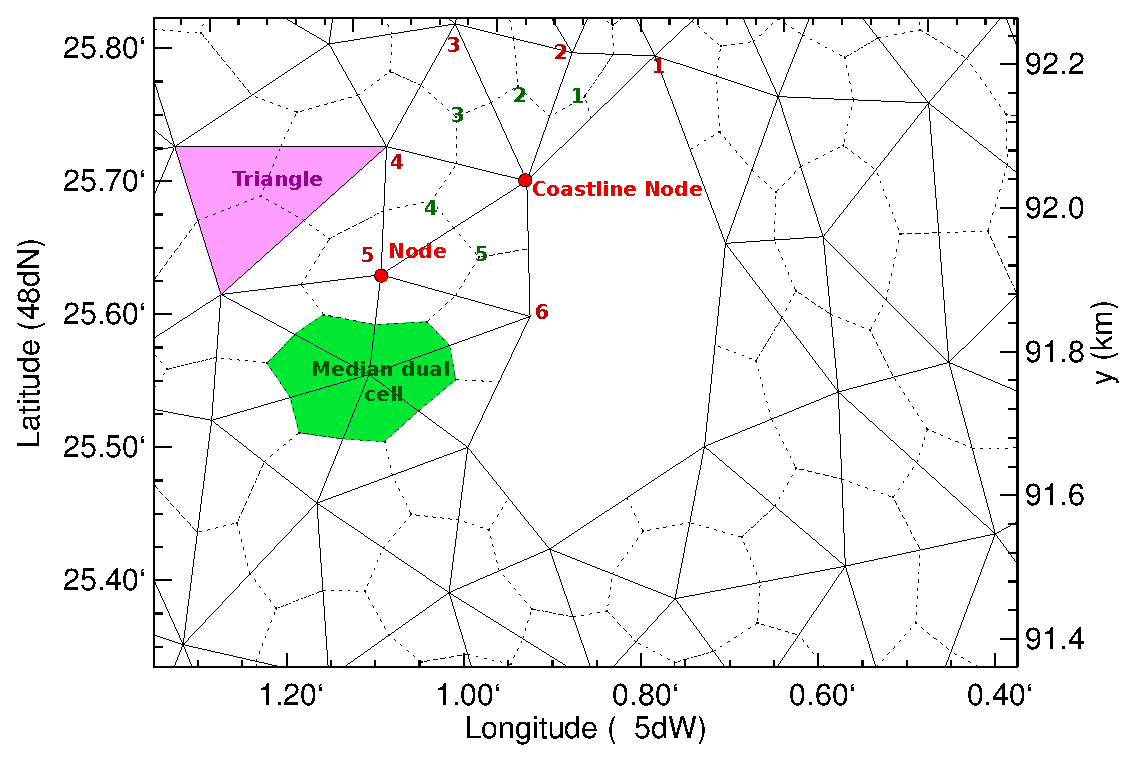
\epsfig{file=./num/grid_triangles.eps,angle=0,width=4.in}
\caption{基于三角形的网格区域示例，本例包含法国 Bannec 小岛。如果水深大于最小水深，岸线节点为活动节点。其特点是相邻节点数（所选示例中为 6）大于相邻三角形数（同一示例中为 5）。}
\label{fig:triangles} \botline
\end{center}
\end{figure}


\begin{figure} \begin{center}
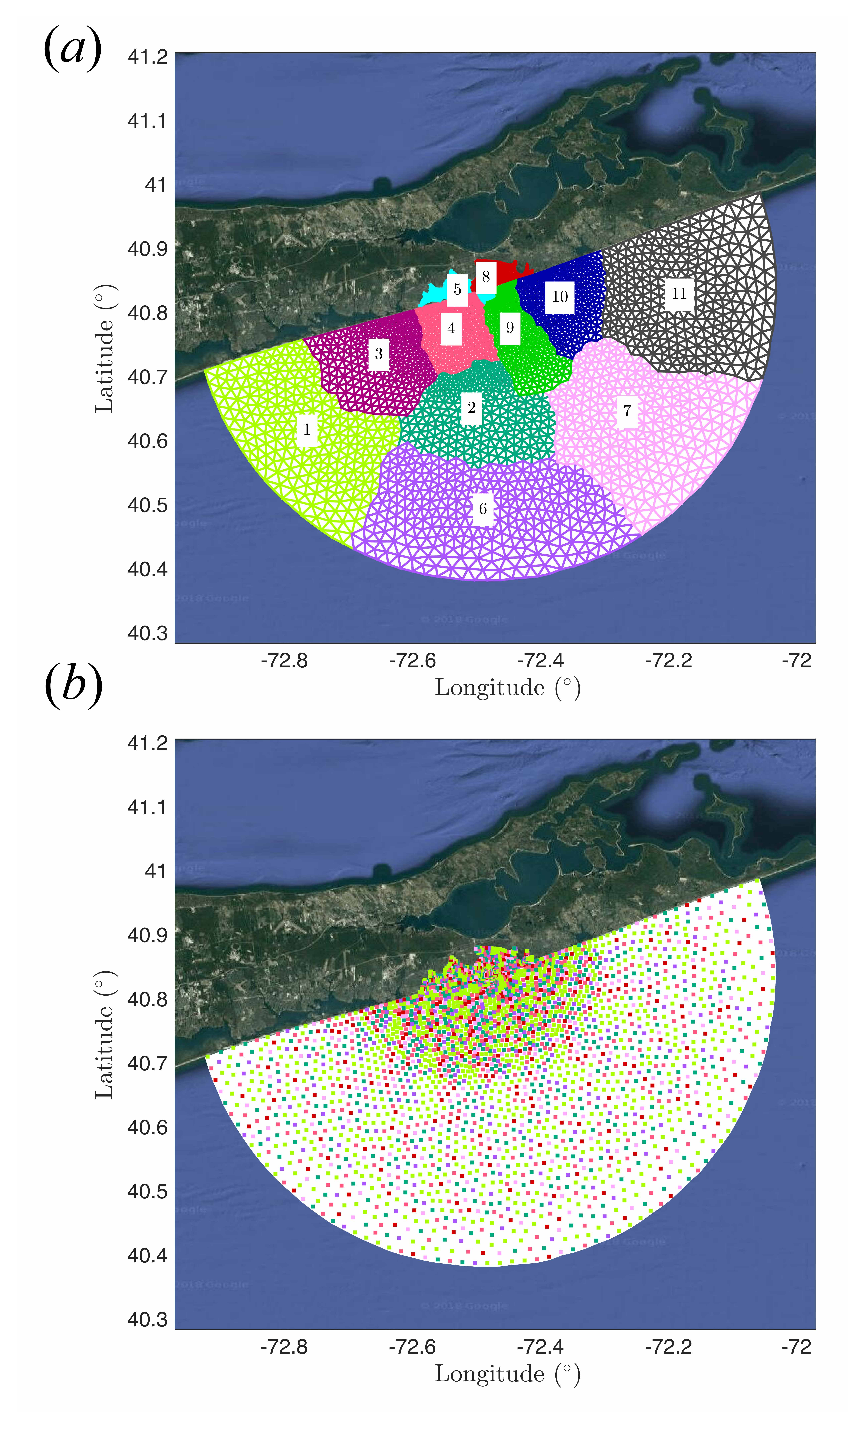
\epsfig{file=./num/DDvsCD.eps,angle=0,width=4.in}
\caption{在 11 个计算核心（以颜色表示）上，区域分解 (a) 与 Card Deck 方法 (b) 的示意差异。该网格约有 3k 个节点，针对纽约 Shinnecock Inlet 构建，取自一个 ADCIRC 示例问题。}
\label{DDvsCD} \botline
\end{center}
\end{figure}

